\documentclass[14pt, a4paper]{article}
\usepackage[russian]{babel}
\usepackage{graphicx}
\usepackage{layout}
\usepackage[14pt]{extsizes}

\setcounter{tocdepth}{4}
\setcounter{secnumdepth}{4}

\usepackage{xcolor}
\usepackage{hyperref}

\usepackage{listings}

 % Цвета для гиперссылок
\definecolor{linkcolor}{HTML}{000000} % цвет ссылок
\definecolor{urlcolor}{HTML}{000000} %цвет гиперссылок

\hypersetup{pdfstartview=FitH,  linkcolor=linkcolor,urlcolor=urlcolor, colorlinks=true}

\definecolor{codegreen}{rgb}{0,0.6,0}
\definecolor{codegray}{rgb}{0.5,0.5,0.5}
\definecolor{codepurple}{rgb}{0.58,0,0.82}
\definecolor{backcolour}{rgb}{0.97,0.97,0.97}

%таблица
\lstdefinestyle{mystyle}{
    backgroundcolor=\color{backcolour},   
    commentstyle=\color{codegreen},
    keywordstyle=\color{magenta},
    numberstyle=\tiny\color{codegray},
    stringstyle=\color{codepurple},
    basicstyle=\ttfamily\footnotesize,
    breakatwhitespace=false,         
    breaklines=true,                 
    captionpos=b,                    
    keepspaces=true,
    frame=single,                                                    
    showspaces=false,                
    showstringspaces=false,
    showtabs=false,                  
    tabsize=2,
    mathescape=true
}

\lstset{style=mystyle}

%Разметка страницы
\oddsidemargin = 0pt
\marginparwidth = 45pt 
\textwidth = 467pt
\textheight = 716pt
\topmargin = 0pt 
\footskip = 30pt 
\headheight = 0pt 
\headsep = 0pt 

\begin{document}
\begin{titlepage}
    \topmargin=216pt
    \newpage
    \hangindent=0.7cm
    \huge ИУ-10\\
    Системное\\
    Программное\\
    Обеспечение\\
    Администрирование Linux\\
    \textbf{Утилиты для жизни в linux \\
    и работы текстовыми файлами}

    \vspace{9cm}

    \begin{center}
        \small\textit{Москва, 2022}
    \end{center}
\end{titlepage}

\section*{На этом уроке}
\addcontentsline{toc}{section}{На этом уроке}
\begin{enumerate}
    \item Разберем утилиты, с помощью которых можно читать текстовые файлы
    \item Познакомимся с текстовыми редакторами vim и nano
    \item Разберем регулярные выражения и их применение
    \item Познакомимся с утилитами для работы с текстовыми файлами
\end{enumerate}


\tableofcontents
\newpage

\section*{Знакомство с текстовыми редакторами} 
\addcontentsline{toc}{section}{Знакомство с текстовыми редакторами}

\subsection*{Утилиты для чтения текстовых файлов} 
\addcontentsline{toc}{subsection}{Утилиты для чтения текстовых файлов}

Для просмотра содержимого файлов существует несколько полезных утилит:

\begin{enumerate}
    \item Команда \textbf{cat (concatenate)} позволяет быстро прочитать содержимое файла, а также склеить
    несколько файлов в один. Например, \colorbox{backcolour}{cat file} выведет на экран содержимое файла с
    именем file. Иногда полезно запускать с опцией -A, чтобы увидеть непечатаемые символы
    \item Программы постраничного просмотра текста \textbf{less} и \textbf{more}. Основное их различие заключается
    в том, что \textbf{less} позволяет просмотр в обе стороны (вверх и вниз) за счёт создаваемого буфера.
    \item  Команда \textbf{tail} позволит вывести на экран заданное количество строк от конца файла или
    содержимое файла в режиме интерактивного просмотра. Например, \colorbox{backcolour}{tail -20 file} -
    покажет последние 20 строк файла file.\colorbox{backcolour}{ tail -f /var/log/syslog} непрерывно выводит на
    экран содержимое файла syslog по мере его обновления. Для прерывания работы tail -f,
    используйте комбинацию Ctrl-C
    \item По аналогии с tail утилита head будет показывать первые линии файла
    \item Текстовые редакторы.     
\end{enumerate}

\subsection*{Текстовый редактор vi/Vim} 
\addcontentsline{toc}{subsection}{Текстовый редактор vi/Vim}


\textbf{Внимание!} \underline{\textit{В силу схожести управления редакторами vi и Vim далее в}} \\
\underline{\textit{тексте рассматриваемработу с Vim}}.\\

\textbf{Vim} — текстовый редактор, обратно совместимый с vi. Он может быть использован для правки
всех видов простого текста. По сравнению с vi, Vim имеет много усовершенствований: многократная
отмена операций, множественность окон и буферов, подсветка синтаксиса, правка командной строки,
автодополнение имён файлов, встроенная справка, визуальное выделение и т. п. Vim имеет большое
количество плагинов, используя которые можно превратить этот редактор в довольно удобную \href{https://ru.wikipedia.org/wiki/Интегрированная_среда_разработки}{IDE}.
Также с редактором устанавливается программа-тренажер \textbf{vimtutor}, которая поможет почувствовать
себя более уверенно в работе с данным редактором.\\

Разберем базовые элементы управления этим редактором.

\newpage

Запускаем редактор командой \textbf{vim myfile}:

\begin{figure}[h]
    \centering
    \scalebox{0.9}{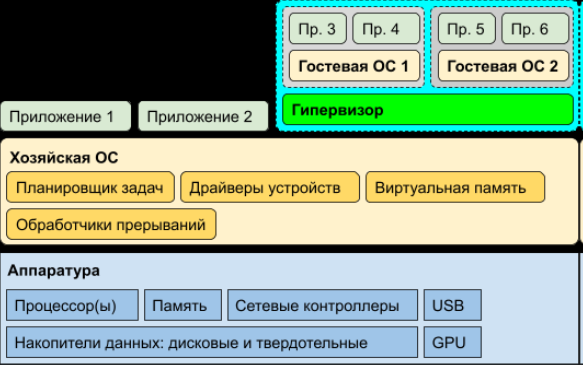
\includegraphics[width=1\textwidth]{1.png}}\\ 
    \label{framework} 
\end{figure}

Vim/vi имеет три режима:
\begin{enumerate}
    \item \textbf{Командный режим}. В этом режиме осуществляется навигация по файлу, выполняются
    редактирующие действия с файлом (удаление символа, копирование, вставка и т. д). \textbf{Важно}:
    команды редактирования вызываются обычными латинскими буквами. Навигация по строкам
    осуществляется либо при помощи клавиш «Вверх», «Вниз», «Влево», «Вправо», либо
    используя буквы: \textbf{k} — вверх, \textbf{j} — вниз, \textbf{h} — влево, \textbf{l} — вправо. Удаление символа под курсором
    — клавиша \textbf{x}. Удаление строки: \textbf{dd} (дважды нажать клавишу d). Пролистывание страниц:
    клавиши \textbf{PgUp}, \textbf{PgDn} или комбинации \textbf{ctrl + F}, \textbf{ctrl + B}.
    \item \textbf{Режим редактирования}. В этом режиме мы можем писать в файл. Для перехода в режим
    редактирования используется одна из команд: клавиша \textbf{i} начнёт редактирование строки с
    текущего положения курсора, клавиша \textbf{a} начнёт редактирование строки со следующего после
    курсора символа, клавиша \textbf{o} начнёт редактирование текста со следующей строки. Вернёмся к
    нашему примеру и переведём редактор в режим редактирования, нажав клавишу \textbf{i}:
\end{enumerate}

\newpage

\begin{figure}[h]
    \centering
    \scalebox{0.67}{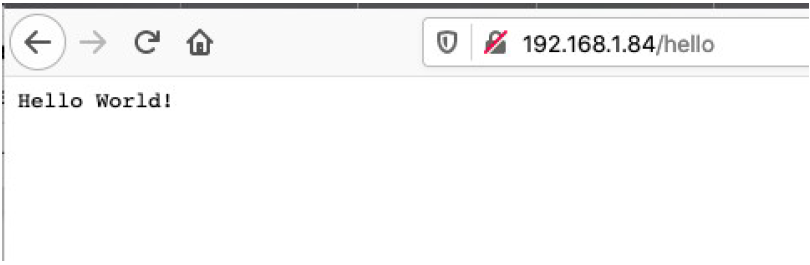
\includegraphics[width=1\textwidth]{2.png}}\\ 
    \label{framework} 
\end{figure}

\noindent \makebox[\linewidth][s]{Курсор начнёт мигать, в левом нижнем углу появится сообщение} \\
\colorbox{backcolour}{\textbf{- - ВСТАВКА - -}} или \colorbox{backcolour}{\textbf{- - INSERT - -}} , что
говорит нам о том, что редактор находится в режиме редактирования и мы можем писать свой текст.

\begin{enumerate}
    \item[3.] \textbf{Режим последней строки} — специальный режим редактора, в котором мы можем передавать
    ему сложные команды, например на сохранение файла, выход из редактора. Для перехода в
    этот режим необходимо проделать следующее: после окончания работы с текстом нажимаем
    клавишу \textbf{Esc} (выходим из режима редактирования), далее нажимаем клавишу «:» (двоеточие)
    и получаем в последней строке редактора приглашение к вводу команд: 
\end{enumerate}

\vspace{-0.5cm}

\begin{figure}[h]
    \centering
    \scalebox{0.68}{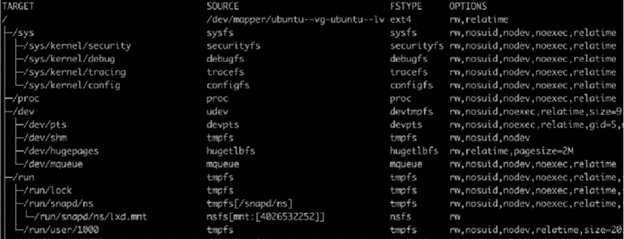
\includegraphics[width=1\textwidth]{3.png}}\\ 
    \label{framework} 
\end{figure}

После двоеточия мы можем использовать следующие команды: \textbf{q} — выйти из редактора, \textbf{q!} — выйти
из редактора без сохранения изменений, \textbf{w} — сохранить файл, \textbf{wq} — сохранить и выйти из
редактора. После ввода нужной команды нажимаем клавишу \textbf{enter}. Более подробно ознакомиться с
командами редактора Vim, как и говорилось выше, поможет программа \textbf{vimtutor}.

\subsection*{Текстовый редактор nano} 
\addcontentsline{toc}{subsection}{Текстовый редактор nano}

\href{https://help.ubuntu.ru/wiki/nano}{\textbf{nano}} — консольный текстовый редактор для Unix и Unix-подобных операционных систем, основанный
на библиотеке curses и распространяемый под лицензией GNU GPL. В настоящее время включён в
дистрибутивы Ubuntu по умолчанию и в установке не нуждается. Более прост и понятен для
начинающего пользователя Linux в сравнении с редакторами vi и Vim. Запускаем редактор следующей
командой: \textbf{nano myfile}.\\

\begin{figure}[h]
    \centering
    \scalebox{0.9}{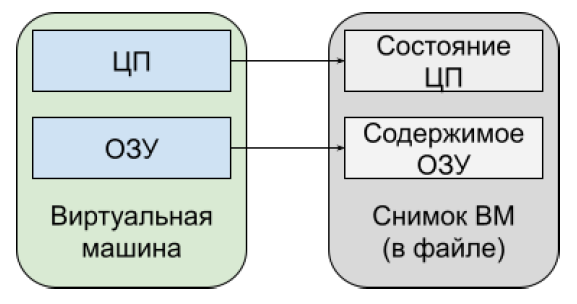
\includegraphics[width=1\textwidth]{4.png}}\\ 
    \label{framework} 
\end{figure}

Сразу после запуска открытый файл становится доступным для редактирования. В отличие от
редактора Vim, у nano нет каких-то особых режимов работы. Ниже области редактирования
располагается панель с наиболее популярными комбинациями клавиш управления редактором.
$\mathtt{\wedge}$ означает клавишу Ctrl. Сохранение файла — комбинация клавиш \textbf{Ctrl + o}, выход из редактора — \textbf{Ctrl
+ x}.

\section*{Перенаправление потоков ввода и вывода} 
\addcontentsline{toc}{section}{Перенаправление потоков ввода и вывода}

Продолжая знакомиться с утилитами для жизни в оболочке Bash, нельзя пропустить стандартные
потоки ввода-вывода. Давайте разберем, что это такое и как мы можем их использовать при
администрировании системы.\\

Одним из принципов UNIX-Way является идея, что каждая программа хорошо отлажена и решает
только одну задачу, но сами программы-утилиты можно комбинировать, что очень часто применяется.
Сейчас мы разберем, каким образом это работает.\\

При запуске каждая программа автоматически открывает 3 специальных файла, которые ещё
называют потоками ввода-вывода. Их различают по номерам файловых дескрипторов (указателей на
файл):

\begin{itemize}
    \item \textbf{0} — стандартный поток ввода (\textbf{STDIN}). Файл, из которого осуществляется чтение данных.
    \item \textbf{1} — стандартный поток вывода (\textbf{STDOUT}). Файл, в который осуществляется запись данных.
    \item \textbf{2} — стандартный поток ошибок (\textbf{STDERR}). Файл, в который осуществляется запись об
    ошибках или сообщения, которые не могут быть записаны в стандартный поток вывода.
\end{itemize}

Информацию из потоков можно перенаправить в любой другой файл, используя следующие символы:

\begin{enumerate}
    \item \textbf{<} — перенаправление стандартного ввода, например, \textbf{<file}. Процесс будет использовать файл
    \textbf{file} как источник данных.
\end{enumerate}

\begin{lstlisting}
user@server:$\sim$$\textdollar$ cat some_text.txt
            
hello World!
            
user@server:$\sim$$\textdollar$ tr [:lower:] [:upper:] < some_text.txt
            
HELLO WORLD!
\end{lstlisting}

\begin{enumerate}
    \item[2.] \textbf{>}, \textbf{>}\textbf{>} — перенаправление стандартного вывода, например, \textbf{>file}. Сообщения от процесса
    будут направлены в файл с именем \textbf{file}. Если файл не существует, он будет создан, в
    противном случае перезаписан. Для записи сообщений в конец файла используется символ
    \textbf{>}\textbf{>}, например, \textbf{>}\textbf{>}\textbf{file}. Сообщения от процесса будут перенаправлены в файл с именем file.
    Если файл не существует, он будет создан. В противном случае сообщения будут дописаны в
    конец файла. \textbf{>} и \textbf{1>} - синонимы, то есть если не указан номер потока, то по умолчанию
    используется первый поток (\textbf{STDOUT}).
\end{enumerate}

\begin{lstlisting}
user@server:$\sim$$\textdollar$ echo "hello world!"

hello world!

user@server:$\sim$$\textdollar$ echo "hello World!" > text_file.txt

user@server:$\sim$$\textdollar$ cat text_file.txt

hello world!

user@server:$\sim$$\textdollar$ echo "Another line!" >> text_file.txt

user@server:$\sim$$\textdollar$ cat text_file.txt

hello world!

Another line!
\end{lstlisting}

\begin{enumerate}
    \item[3.] \textbf{2>}, \textbf{2>}\textbf{>} — перенаправление стандартного потока ошибок, например, \textbf{2>file}. Сообщения об
    ошибках процесса будут направлены в файл с именем \textbf{file}. Если файл не существует, он будет
    создан, в противном случае перезаписан. Для записи сообщений в конец файла используется
    символ \textbf{2>}\textbf{>}, например, \textbf{2>}\textbf{>}\textbf{file}. Сообщения об ошибках процесса будут перенаправлены в
    файл с именем file. Если файл не существует, он будет создан, в противном случае сообщения
    будут дописаны в конец файла.
\end{enumerate}

\begin{lstlisting}
user@server:$\sim$$\textdollar$ some_text.txt

some_text.txt: command not found

user@server:$\sim$$\textdollar$ some_text.txt 2> err_text.txt

user@server:$\sim$$\textdollar$ cat err_text.txt

some_text.txt: command not found
\end{lstlisting}

\begin{enumerate}
    \item[4.] \textbf{2>\&1} — позволит объединить поток ошибок (stderr) и стандартный вывод (stdout) и
    перенаправить данные в другой файл.
\end{enumerate}

\noindent Стандартные потоки можно перенаправлять не только в файлы, но и на ввод другим процессам. Такое
перенаправление называют конвейер (pipeline), в нём используется специальный символ pipe «|»
(вертикальная черта). Например, \colorbox{backcolour}{command-1 | command-2|...|command-n} перенаправит результат
работы команды \colorbox{backcolour}{command-1} на ввод другой команде — \colorbox{backcolour}{command-2}, которая, в свою очередь,
перенаправит результат своей работы на ввод следующей команде. Такое перенаправление очень
часто используется в работе с командной строкой Linux. Например, используя такое
перенаправление, мы можем подсчитать количество объектов в текущем каталоге.

\vspace{0.5cm}

\begin{lstlisting}
user@server:$\sim$$\textdollar$ ls -l | wc -l

30
\end{lstlisting}

\section*{Утилиты для работы с текстом} 
\addcontentsline{toc}{section}{Утилиты для работы с текстом}

\subsection*{Регулярные выражения} 
\addcontentsline{toc}{subsection}{Регулярные выражения}

Регулярные выражения — инструмент, предназначенный для поиска, а также обработки текста по
заданному шаблону. Используя регулярные выражения, мы можем изменять текст, искать строки в
файле, фильтровать список файлов согласно каким-то условиям и т. д. Регулярные выражения —
неотъемлемая часть командного интерпретатора bash. Они постоянно применяются в работе с
командной строкой.\\

Регулярные выражения можно разделить на два типа: \textbf{POSIX} и \textbf{PCRE} (perl-совместимые регулярные
выражения). Основное различие — набор используемых символов. В bash используются регулярные
выражения PO- SIX, которые делятся на два типа: BRE (базовые регулярные выражения) и ERE
(расширенные регулярные выражения). Они различаются используемыми символами: в ERE их
больше, и синтаксис ближе к регулярным выражениям PCRE.\\

\noindent В регулярных выражениях используется два типа символов:
\begin{enumerate}
    \item \textbf{Обычные символы} — буквы, цифры, знаки препинания — всё, из чего состоят слова и
    строки.
    \item \textbf{Метасимволы} — специальные символы, при помощи которых усиливается регулярное
    выражение. Эти символы используются для замены других символов или их
    последовательностей, например для группировки символов.
\end{enumerate}

\vspace{0.2cm}

\noindent Метасимволы также можно разделить на группы:
\begin{itemize}
    \item \textbf{Символы-якоря} — символы, определяющие позицию шаблона в тексте. \textbf{$\string^$} (символ «каретка»)
    обозначает начало строки, \textbf{\$} (знак доллара) обозначает конец строки.
    \item \textbf{Символы-модификаторы} — символы, определяющие количество повторов предыдущего
    символа или набора символов.\\
\end{itemize}

\noindent \href{https://losst.pro/regulyarnye-vyrazheniya-linux}{Основные символы-модификаторы}:
\begin{itemize}
    \item \textbackslash \ \ - \ с обратной косой черты начинаются буквенные спецсимволы, также она применяется,
    если нужно использовать спецсимвол в виде знака препинания (экранирование);
    \item * — указывает, что предыдущий символ может повторяться 0 или больше раз;
    \item + — указывает, что предыдущий символ должен повториться больше 1 или больше раз;
    \item ? — предыдущий символ может встречаться 0 или 1 раз;
    \item \{n\} — указывает сколько раз (n) нужно повторить предыдущий символ;
    \item \{N,n\} — предыдущий символ может повторяться от N до n раз;
    \item . — любой символ, кроме перевода строки;
    \item $[az]$ — любой символ, указанный в скобках;
    \item х|у — символ x или символ y;
    \item $[$\string^$az]$ — любой символ, кроме тех, что указаны в скобках;
    \item $[a-z]$ — любой символ из указанного диапазона;
    \item $[$\string^$a-z]$ — любой символ, которого нет в диапазоне;
    \item \textbackslash b — обозначает границу слова с пробелом;
    \item \textbackslash B — означает, что символ должен не быть окончанием слова;
    \item \textbackslash d — означает, что символ — цифра;
    \item \textbackslash D — нецифровой символ;
    \item \textbackslash n — символ перевода строки;
    \item \textbackslash s — любой пробельный символ: пробел, табуляция и так далее;
    \item \textbackslash S — любой непробельный символ;
    \item \textbackslash t — символ табуляции;
    \item \textbackslash v — символ вертикальной табуляции;
    \item \textbackslash w — любой буквенный символ, включая подчёркивание;
    \item \textbackslash W — любой буквенный символ, кроме подчёркивания;
    \item \textbackslash uXXX — конкретный указанный символ Unicode.
\end{itemize}

Для работы с регулярными выражениями в bash можно применять изученные ранее утилиты: grep,
SED и AWK.

\subsection*{grep} 
\addcontentsline{toc}{subsection}{grep}

\href{https://ru.wikipedia.org/wiki/Grep}{\textbf{Grep}} находит на вводе целые строки, отвечающие заданному текстовому шаблону, и выводит их, если
вывод не отменён специальным ключом. Grep работает с регулярными выражениями POSIX (BRE),
но у него есть модификация egrep, которая позволяет расширенный синтаксис (ERE). Утилита имеет
множество параметров, об этом более подробно можно прочитать на страницах справочного
руководства man grep. Наиболее используемые опции:

\begin{itemize}
    \item \textbf{grep -ir} — искать заданный шаблон без учёта регистра, рекурсивно включая вложенные
    каталоги, например \colorbox{backcolour}{grep -ir error /var/log/*} будет искать строки, содержащие в себе
    слово error, в каталоге /var/log, включая вложенные подкаталоги;
\end{itemize}

\begin{lstlisting}
user@server:$\sim$$\textdollar$ grep -ir error
/var/log/*
                                                                  16:28:1
URL:http://ftpmaster.internal/ubuntu/pool/main/libg/libgpg-error/libgpg-e
1rror0_1.37-1_amd64.deb                [58004/58004]                    ->
"/build/chroot//var/cache/apt/archives/partial/libgpg-error0_1.37-1_amd64.
deb"
[1]

/var/log/bootstrap.log:Selecting      previousl     unselecte     packag
libgpg-error0:amd64.

/var/log/bootstrap.log:Preparing to unpack .../libgpg-error0_1.37-1_amd64.
deb ...

/var/log/bootstrap.log:Unpacking libgpg-error0:amd64 (1.37-1) ...

/var/log/bootstrap.log:Setting up libgpg-error0:amd64 (1.37-1) ...

...
\end{lstlisting}

\begin{itemize}
    \item \textbf{grep -P} будет использовать расширенные возможности регулярных выражений;
\end{itemize}

\begin{lstlisting}
user@server:$\sim$$\textdollar$ grep -P 'Jan\s\d{2}\s20' /var/log/syslog

Jan 10 20:14:59 server snapd[614]: storehelpers.go:551: cannot refresh: 
snap has no updates available: "core18", "lxd"

Jan 10 20:15:09 server systemd[1]: Reloading.

Jan  10  20:15:09  server  systemd[1]:  /lib/systemd/system/dbus.socket:5:
ListenStream= references a path below legacy directory /var/run/, updating
/var/run/dbus/system_bus_socket -> /run/dbus/system_bus_socket; please 
update the unit file accordingly.

Jan 10 20:15:09 server systemd[1]: Reloading.

...
\end{lstlisting}

\begin{itemize}
    \item \textbf{grep -v} исключит из поиска строки, содержащие шаблон, например \colorbox{backcolour}{cat /var/log/syslog
    | grep -v} named выведет на экран содержимое файла \textbf{/var/log/syslog}, за исключением строк,
    содержащих в себе слово \textbf{named}.
\end{itemize}

\begin{lstlisting}
user@server:$\sim$$\textdollar$ cat /var/log/syslog |grep -v named

Jan 10 14:17:33 server systemd[1]: logrotate.service: Succeeded.

Jan 10 14:17:33 server systemd[1]: Finished Rotate log files.

Jan 10 14:17:33 server systemd[1]: fstrim.service: Succeeded.

Jan 10 14:17:33 server systemd[1]: Finished Discard unused blocks on 
filesystems from /etc/fstab.

Jan 10 14:17:33 server systemd[1]: man-db.service: Succeeded.

Jan 10 14:17:33 server systemd[1]: Finished Daily man-db regeneration.

...
\end{lstlisting}

\subsection*{SED} 
\addcontentsline{toc}{subsection}{SED}

\href{https://habr.com/ru/company/ruvds/blog/327530/}{\textbf{SED}} — потоковый текстовый редактор. Позволяет редактировать потоки данных на основе заданных
правил. С помощью SED можно провести простые операции по поиску и замене слов в тексте. В
общем случае синтаксис выглядит следующим образом:\colorbox{backcolour}{ sed ‘s/шаблон/замена/g’ file}. Здесь \textbf{s}
— искать; \textbf{шаблон} — то, что ищем; \textbf{замена} — то, на что меняем текст; \textbf{g} — глобально, то есть во всём
файле с именем \textbf{file}.\\

Простой пример: \colorbox{backcolour}{sed ‘s/test/text/g’ file} найдёт все вхождения слова \textbf{test} в файле \textbf{file} и
заменит на слово \textbf{text}, при этом результат работы выведет на экран, не изменяя основного файла.

\vspace{0.3cm}

\begin{lstlisting}
user@server:$\sim$$\textdollar$ cat file

test

test something

another tessssst

test

test hello

user@server:$\sim$$\textdollar$ sed 's/test/text/g' file

text

text something

another tessssst

text

text hello

\end{lstlisting}
\vspace{0.2cm}

Если мы хотим сразу применить изменения, то следует команде \textbf{sed} передать параметр \textbf{i} (\textbf{sed -i}).
Данный параметр позволяет сразу править файл: \colorbox{backcolour}{sed -i ‘s/test/text/g’ file}.

\subsection*{AWK} 
\addcontentsline{toc}{subsection}{AWK}

\textbf{AWK} — более мощная, чем SED, утилита для обработки потока данных. С точки зрения AWK данные
разбиваются на наборы полей, то есть наборы символов, разделённых разделителем. AWK — это
практически полноценный язык программирования, в котором есть свои переменные, операторы
выбора и циклы. AWK — родоначальник языка perl.\\

В AWK используются переменные трёх типов: числовые (\textbf{x=5}), строковые (\textbf{x=abc}) и переменные поля,
которые обозначаются \textbf{\$1}, \textbf{\$2} и т. д. В отличие от скрипта bash, они означают номера полей, на
которые разбита строка.\\

AWK можно использовать как самостоятельный язык для написания сценариев или вызывать его из
командной строки для обработки потока 
\makebox[\linewidth][s]{данных. Вызов происходит следующим образом:} 
\colorbox{backcolour}{поток\_данных | awk '{ скрипт\_обработки\_данных}'}. Здесь \textbf{поток\_дан-} \\
\textbf{ных} — любая команда ОС или скрипт, результат работы которого будем передавать через \textbf{pipe (|)} на обработку AWK.\\

\colorbox{backcolour}{‘{скрипт\_обработки\_данных}’} — скрипт, написанный с использованием синтаксиса AWK.
Например, \colorbox{backcolour}{ls -l | awk ‘{ print \$1 }’} выведет на экран первый столбец из вывода команды ls -l.

\vspace{0.3cm}

\begin{lstlisting}
@server:$\sim$$\textdollar$ ls -la | awk '{print $\textdollar$1 }'

total

drwxr-xrx

drwxr

-rw-r--r-

-drwxr

xr-x

-rw

-rw-r--r--

-rw-r--r--

\end{lstlisting}

\subsection*{cut,sort,tr} 
\addcontentsline{toc}{subsection}{cut,sort,tr}

Последние команды, которые хотелось бы упомянуть (и продемонстрировать несколько примеров
использования конвейера), - это cut, sort и tr. \textbf{cut} предназначен для фильтрации вывода. \textbf{sort}
предназначен для сортировки вывода. А \textbf{tr} - для перевода.\\

Команде cut необходимо передать делимитер (опция d) для разделения различных элементов в
строке и номер элемента (опция f) для отображения.
\vspace{0.3cm}

\begin{lstlisting}
root@server:$\sim$# cut -f 3 -d : /etc/passwd

0

1

2

...

41

65534

100

\end{lstlisting}
\vspace{0.2cm}

Воспользуемся pipe и утилитой sort.

\vspace{0.3cm}

\begin{lstlisting}
root@server:$\sim$# cut -f 3 -d : /etc/passwd | sort

0

1

10

100

1000

1001

1002

...

root@server:$\sim$# cut -f 3 -d : /etc/passwd | sort -n

0

1

2

3

\end{lstlisting}
\vspace{0.2cm}

Сама по себе команда sort не понимает, что перед ней числа, поэтому мы получили не совсем
ожидаемый результат. Ключ -n привел все в порядок.\\

И последняя утилита tr поможет с преобразованием текста, для этого возьмем первое поле с логином.

\vspace{0.3cm}
\begin{lstlisting}
root@server:$\sim$# cut -f 1 -d : /etc/passwd | tr [:lower:] [:upper:]

ROOT

DAEMO

N BIN

SYS

SYNC

GAMES

MAN

\end{lstlisting}



\section*{Практическое задание} 
\addcontentsline{toc}{section}{Практическое задание}

\begin{enumerate}
    \item Создать файл с наполнением, используя несколько способов. Использовать изученные на
    занятии текстовые редакторы для наполнения файлов произвольными данными.
    \item Попробовать вывести с помощью cat содержимое всех файлов в директории \textbf{/etc} (cat /etc/*).
    Направить ошибки в отдельный файл в вашей домашней директории. Сколько объектов \textbf{не}
    удалось прочесть?
    \item Использовать команду cut на вывод длинного списка каталога, чтобы отобразить только права
    доступа к файлам. Затем отправить в конвейере этот вывод на sort и uniq, чтобы
    отфильтровать все повторяющиеся строки. Потом с помощью wc подсчитать различные типы
    разрешений в этом каталоге. \textbf{\textit{Попробовать}} убрать из подсчета строку \textbf{total}.
    \item * В ОС Linux скрытыми файлами считаются те, имена которых начинаются с точки. Сколько
    скрытых файлов в вашем домашнем каталоге?
    \item * Используя дополнительный материал, настроить авторизацию по SSH с использованием
    ключей.
\end{enumerate}

\section*{Глоссарий} 
\addcontentsline{toc}{section}{Глоссарий}

\underbar{\textbf{Консольные текстовые редакторы}} — редакторы текста для командной строки в ОС Linux.
\href{https://losst.ru/luchshie-tekstovye-redaktory-linux}{Небольшой обзор редакторов.}\\

\noindent \href{https://ru.wikipedia.org/wiki/Стандартные_потоки}{\underbar{\textbf{Стандартные потоки}}} — специальный тип потоков, имеющих свой номер (дескриптор) и
предназначенных для выполнения стандартных функций: ожидание команд пользователя, вывод
данных на экран, вывод сообщений об ошибках на экран.\\

\noindent \href{https://ru.wikipedia.org/wiki/Конвейер_(Unix)}{\underbar{\textbf{Конвейер (pipeline)}}} — набор процессов, для которых реализована следующая схема: вывод
результата работы одного процесса передаётся на ввод другому процессу.\\

\noindent \href{https://ru.wikipedia.org/wiki/Аутентификация}{\underbar{\textbf{Аутентификация}}} — процедура проверки подлинности, например сравнением введённого пароля
пользователя с паролем, сохранённым в базе данных паролей.\\

\noindent \href{https://losst.pro/regulyarnye-vyrazheniya-linux}{\underbar{\textbf{Регулярные выражения}}} — инструмент для поиска текста по шаблону, обработки и изменения строк,
который можно применять для следующих задач: поиск и замена текста в файле, проверка строки на
соответствие шаблону и т. д.

\section*{Дополнительные материалы} 
\addcontentsline{toc}{section}{Дополнительные материалы}

\begin{enumerate}
    \item \href{https://habr.com/ru/post/115825/}{\textit{Регулярные выражения}}
    \item \href{http://rus-linux.net/MyLDP/consol/sed.html}{\textit{SED}}
    \item \href{http://rus-linux.net/MyLDP/consol/awk.html}{\textit{AWK}}
    \item \href{http://xgu.ru/wiki/Стандартные_потоки_ввода/вывода}{\textit{Потоки ввода/вывода}}
    \item \href{https://losst.pro/avtorizatsiya-po-klyuchu-ssh}{\textit{Авторизация по ключу}}
    \item \href{https://rtfm.co.ua/putty-nastrojka-avtorizacii-ssh-po-klyuchu/}{\textit{Настройка авторизации по ключу, используя программу PuTTY}}
    \item \href{https://losst.pro/luchshie-tekstovye-redaktory-linux}{\textit{Небольшой обзор редакторов}}
\end{enumerate}

\section*{Используемые источники} 
\addcontentsline{toc}{section}{Используемые источники}

\href{https://losst.pro/regulyarnye-vyrazheniya-linux}{\textit{Регулярные выражения в Linux}}\\

\noindent \href{https://www.linuxcenter.ru/lib/books/kostromin}{\textit{Костромин В. Linux для пользователя}}\\

\noindent \href{https://help.ubuntu.ru/wiki/vim}{\textit{Статья, посвящённая текстовым редакторам vi/Vim}}\\


\end{document}
